\chapter{Teoretický základ}
	V následující kapitole jsou nejdříve rozebrány základní termíny, které jsou použíty v~práci. Následuje základní popis existujících algoritmů, kde je \gls{gloss:CYK} algoritmus popsán podrobněji a to včetně transformací do Chomského normální formy (dále jen \gls{gloss:CNF}).
	
	\section{Formální jazyky a gramatiky}
		\label{sec:formalLanguagesAndGrammars}
		Pro popis strukturovaného textu se využívají formální jazyky \cite{Meduna:2014:FLC:2636678}. Počátky sahají do 50. let 20. století, kdy Noam Chomsky vytvořil na základě poznatků Alana Turinga, Axele Thuea a Emila Posty definici formální gramatiky. Formální gramatiky se využívají především v teoretické informatice pro popis struktury programovacích jazyků a výpočtových modelů \cite{Havill:2015:DCS:2855048}.
		
		Vzhledem k~tomu, že knihovna bude pracovat se základními elementy teorie jazyků (konkrétně reprezentace gramatik), považujeme za nutné na úvod uvést základní definice z~důvodu jejich sjednocení, které se v~různých publikacích mohou lišit. Definice vycházejí z~materiálů Gerharda Jägera a Jamese Rogerse \cite{Jager2012}.
	
		\paragraph{Symbol}
		je elementární, dále nedělitelný objekt. Může se jednat o~písmeno, číslo, ale i~tón, frekvenci či jinou námi definovanou entitu.
		\paragraph{Abeceda}
		je konečná množina symbolů.
		\paragraph{Slovo}
		je sekvence symbolů z~abecedy.
		\paragraph{Formální jazyk}
		je množina slov. Množina může být i~nekonečná.
		
		\vspace{1em}
		
		Formální gramatika umožňuje popsat formální jazyk konečným výrazem bez toho, aniž bychom jej museli definovat výčtem \cite{Meduna:2014:FLC:2636678}. Pro definici gramatiky budeme potřebovat následující pojmy:
		
		\paragraph{Terminál}
		je symbol formálního jazyka. Dále v~textu budeme množinu terminálů (či terminálních symbolů) označovat jako \MathSymb{T}, prvky této množiny malými písmeny.
		\paragraph{Neterminál}
		je symbol abecedy, která je rozdílná od abecedy terminálů. Abecedy terminálů a neterminálů jsou navzájem disjunktní. Množinu neterminálů (nebo také neterminálních symbolů) označujeme jako \MathSymb{N}, prvky této množiny velkými písmeny.
		\paragraph{Počáteční symbol}
		je konkrétní symbol z~množiny neterminálů. Někdy se počáteční symbol označuje i~jako symbol startovací. Nebude-li v~textu uvedeno jinak, budeme jako počáteční symbol uvažovat neterminál \MathSymb{S}.
		\paragraph{Epsilon}
		je speciální symbol, který označuje slovo nulové délky. Dále v~textu značíme jako \Eps.
		\paragraph{Iterace}
		je opakování symbolu (resp. slova) 0 až neomezeně mnohokrát. Značíme $x^{\ast}$ (například $a^{\ast} = \left\{ \varepsilon, a, aa, \dots, a^n \right\}, n\ge 0  $).
		\paragraph{Pravidlo}
		je prvek kartézského součinu 
		$\TermNontermIter
			\times
		\TermNontermIter$.
		V~práci budeme pravidla psát ve tvaru $\alpha\rightarrow\beta$, kde $(\alpha,\beta)$ je prvek zmíněného kartézského součinu. Zápis chápeme jako \enquote{$\alpha$ může být nahrazeno $\beta$}.
		\paragraph{Gramatika}
		je čtveřice \GrammarDef, kde \MathSymb{R} je množina pravidel gramatiky a \MathSymb{S} je počáteční symbol.
		
		\vspace{1em}
		
		Pro další práci budeme potřebovat definovat pojmy související s~převodem gramatik a~prací s~nimi \cite{Meduna:2014:FLC:2636678}.
		
		\paragraph{Přímá derivace}
		je nahrazení $\gamma\alpha\delta$ slovem $\gamma\beta\delta$, kde 
		$\alpha,\beta,\gamma,\delta\in
			\TermNontermIter$.
		Ve zbytku práce budeme předpokládat pouze derivace nad konkrétní gramatikou. Pro přímou derivaci nad gramatikou musí v~gramatice existovat pravidlo ve tvaru $\alpha\rightarrow\beta$. Přímou derivaci budeme značit jako
		$\gamma\alpha\delta \;
			{\Rightarrow}^{1} 
		\; \gamma\beta\delta$.
		\paragraph{Nultá derivace}
		je reflexivní uzávěr přímé derivace. Každý prvek je v~relaci nulté derivace sám se sebou a~značíme 	
		$\alpha\;
			{\Rightarrow}^{0} 
		\; \alpha$
		\paragraph{\textit{K}-tá derivace}
		je opakované použití přímé derivace. Výsledek $k-1$ derivace využijeme pro výpočet $k$-té derivace zřetězením s přímou derivací. Označujeme jako 	
		$\alpha\;
			{\Rightarrow}^{k} 
		\; \beta$
		a definujeme indukcí.
		$$(\alpha\;
			{\Rightarrow}^{k} 
		\; \beta)
		\Leftrightarrow
		((\alpha\;
			{\Rightarrow}^{k-1} 
		\; \gamma)
		\wedge
		(\gamma\;
			{\Rightarrow}^{1} 
		\; \beta))$$
		\paragraph{Derivace}
		je v~práci chápána jako tranzitivní a reflexivní uzávěr přímé derivace. Budeme značit jako
		$\alpha\;
			{\Rightarrow}
		\; \beta$
		a jedná se o ekvivalent zápisu
		$\alpha\;
			{\Rightarrow}^{i} 
		\; \beta$
		pro $i\ge0$.
		\paragraph{Větná forma}
		je řetězec $\alpha$ vygenerovaný gramatikou \GrammarDef, jestli\-že existuje derivace $S\Rightarrow\alpha,\alpha\in\TermNontermIter$.
		\paragraph{Věta}
		je větná forma, která obsahuje pouze terminální symboly. Dále v práci je věta a slovo jazyka považováno za synonyma.
		\paragraph{Generovaný jazyk \MathSymb{L}}
		gramatikou  \GrammarDef\space je takový jazyk, jenž obsahuje všechny věty generované gramatikou. 
		$$L(G)=\left\{ w:w\in{T}^{*},\exists S \Rightarrow w \right\}$$
		\paragraph{Ekvivalentní gramatiky}
		jsou gramatiky $G_1$ a $G_2$, které generují stejný jazyk. Formálně $L(G_1)=L(G_2)$.
		
		\vspace{1em}
		
		Noam Chomsky rozdělil gramatiky do čtyř kategorií \cite{Meduna:2014:FLC:2636678}. Se zvyšující se kategorií se zvyšuje komplexita gramatiky a tím i~její obecnost. Tyto kategorie se označují jako \MathSymb{typ 0}, \MathSymb{typ 1}, \MathSymb{typ 2} a \MathSymb{typ 3}, kde \MathSymb{typ 0} je z~nich nejobecnější \cite{chomsky59}. 
		Jazyky generované konkrétnějšími skupinami gramatik jsou podmnožinou jazyků generovaných gramatikami obecnějšími. 
		Jazyky, které tyto gramatiky popisují, se nazývají \MathSymb{rekurzivně spočetné} (pro \MathSymb{Typ 0} gramatiky), \MathSymb{kontextové}, \MathSymb{bezkontextové} a \MathSymb{regulární} (pro \MathSymb{Typ 3} gramatiky). 
		V~některých zdrojích toto pojmenování \enquote{zdědily} i~samotné gramatiky, proto budeme v~dále textu označovat synonymem
		\begin{itemize}
			\item \MathSymb{regulární gramatiky} jako gramatiky typu \MathSymb{3},
			\item \MathSymb{bezkontextové gramatiky} jako gramatiky typu \MathSymb{2},
			\item \MathSymb{kontextové gramatiky} jako gramatiky typu \MathSymb{1},
			\item \MathSymb{neomezené gramatiky} jako gramatiky typu \MathSymb{0}.
		\end{itemize}
		
		Jednotlivé typy gramatik se mezi sebou liší tvarem pravidla. Z~původní definice kartézského součinu $\TermNontermIter\times\TermNontermIter$ povoluje každá ze skupin pouze podmnožinu pravidel.
		\begin{itemize}
			\item Regulární gramatiky povolují pouze pravidla typu $A\rightarrow a$, $A\rightarrow aB$ a~eventuálně pravidlo $S\rightarrow\varepsilon$, pokud se počáteční symbol \MathSymb{S} nevyskytuje na pravé straně pravidla.
			\item Bezkontextové gramatiky povolují pravidla typu $A\rightarrow\TermNontermIter$.
			\item Kontextové gramatiky povolují pravidla typu $\gamma{A}\delta\rightarrow\gamma\alpha\delta$, kde
			$\alpha\in\TermNonterm\TermNontermIter$, ${\gamma,\delta\in\TermNontermIter}$ 
			a~eventuálně $S\rightarrow\varepsilon$, pokud počáteční symbol \MathSymb{S} není na pravé straně pravidla.
			\item Neomezené gramatiky povolují pravidla typu 
			$$\TermNontermIter X \TermNontermIter 
			\rightarrow 
			\TermNontermIter$$
			kde \Term{X} je neterminál
		\end{itemize}
	
	 	Všimněme si, že bezkontextová gramatika není nutně gramatikou kontextovou, nicméně jazyk generovaný libovolnou bezkontextovou gramatikou lze popsat gramatikou kontextovou.
		Ke každé kategorii byl přiřazen i~model, který je schopen všechny jazyky dané kategorie rozpoznat.
		Dále v~textu bude zmíněn pouze zásobníkový automat, který je přiřazen k~bezkontextovým gramatikám \cite{Meduna:2014:FLC:2636678}. Zbývající modely jsou vzhledem k~zaměření práce nepodstatné.
		
		
	\section{Bezkontextové gramatiky}
		Dále se v~práci zaměříme pouze na gramatiky bezkontextové. Důvod je ten, že regulární gramatiky mají malou vyjadřovací schopnost a nedovedou popsat běžné jazykové konstrukce. Pro příklad uveďme párování složených závorek pro jazyky založených na syntaxi jazyka C.
		
		\begin{proof}[Důkaz, že regulární jazyky nejsou schopny popsat párování závorek \cite{SestakovaCvicebnice}:]	
			\begin{flushleft}
				$ $\linebreak
				$$L=\Big\{ 
				{\left\{\right.}^n 
				{\left.\right\}}^n;
				n\ge0 
				\Big\}$$
				\begin{enumerate}
					\item Předpokládáme, že jazyk \MathSymb{L} je regulární. Pak na základě pummping lemmatu \cite{DBLP:journals/corr/PettorossiP17} musí platit:
					$$
					\left( \exists p \ge 1 \right)
					\left( \forall w \in L \right)	
					|w| \ge p $$
					$$\Rightarrow$$ 
					$$
						\left( \exists x,y,z \in \Iter{T} \right)
						\left( w = xyz \wedge |xy| \le p \wedge |y| \ge 1 \wedge (\forall k \ge 0)x{y}^{k}z \in L \right)
					$$
					\item
					Ukážeme, že platí negace této vlastnosti. Neboli, že
					$$
					(\forall p \ge 1)
					(\exists w \in L)
					[
						|w| \ge p \wedge 
						(\forall x,y,z \in \Iter{T})
						$$
						$$
						(
							(w = xyz \wedge |xy| \le p \wedge |y| \ge 1)
							\Rightarrow
							(\exists k \ge 0)xy^kz \notin L
						)
					]
					$$
					Tím dostaneme spor s předpokladem, že jazyk \MathSymb{L} je regulární. Důkaz neregularity jazyka \MathSymb{L} tak bude hotov.
					\begin{enumerate}
						\item 
						$\forall p \ge 1$ volíme větu \MathSymb{w} tak, aby
						$w \in L \wedge |w| \ge p: w={\left\{\right.}^{p+1} {\left.\right\}}^{p+1}$.
						\item 
						Najdeme všechny rozklady $xyz$ pro zvolenou větu \MathSymb{w} tak, aby 
						$$w=xyz \wedge |xy| \le p \wedge |y| \ge 1$$.
						\begin{tabular}{l l}
							$x={\left\{\right.}^{r}$ & $r \ge 0$ \\
							$y={\left\{\right.}^{s}$ & $s \ge 1, r+s \le p$ \\
							$z={\left\{\right.}^{t} {\left.\right\}}^{p+1}$ & $t \ge 0, r+s+t=p+1$
						\end{tabular}
						\item 
						Volíme \MathSymb{k} tak, aby $k \ge 0 \wedge xy^kz \notin L$:
						$$k = 0: xy^kz=xy^0z=
						{\left\{\right.}^{r}{\left\{\right.}^{t} {\left.\right\}}^{p+1}=
						{\left\{\right.}^{r+t} {\left.\right\}}^{p+1}
						\notin L$$
						protože $r+t = p + 1 - s \wedge s \ge 1 \Rightarrow r+t < p + 1$.
						\item 
						Dostali jsme spor s předpokladem, že jazyk \MathSymb{L} je regulární jazyk. Jazyk \MathSymb{L} tedy není regulární. 
					\end{enumerate}
				\end{enumerate} 
			\end{flushleft}
		\end{proof}
	
		Na druhé straně parsování kontextových jazyků je příliš náročné. To je způsobeno tím, že kontextové jazyky jsou nedeterministické a z~toho přímo vyplývá exponenciální složitost parsování \cite{DBLP:journals/corr/LaurentM16}. Nepoužití kontextových jazyků s~sebou nese komplikace, protože většina jazyků využívá vlastnosti kontextových gramatik. Pro příklad uveďme deklaraci proměnné před jejím použití \cite{Lai2008}.
		
		Drtivá většina dnešních parserů je založených na bezkontextových gramatikách \cite{Sikkel1997}. Ty mají dostatečnou abstrakci pro popis běžně používaných konstrukcí programovacích jazyků. Omezení, které bezkontextové gramatiky mají, a díky kterým nelze popsat všechny jazykové konstrukce, se řeší přídavným kódem přímo v parseru, dodatečným zpracováním výstupu parseru nebo odklonem od formální definice gramatiky a její modifikací pro účely parsování konkrétního programovacího jazyka. Pro příklad uveďme deklaraci proměnné před jejím použitím, řešeno tabulkou symbolů během procesu parsování, nebo if-else problém \cite{Abrahams:1966:FSD:365813.365821} řešený v případě LL parserů úpravou LL parsovací tabulky (viz kapitola \ref{sec:LLgrammars}) \cite{Aho:1986:CPT:6448}.
		
		\vspace{1em}
		
		Bezkontextové gramatiky můžeme dále rozdělit na několik skupin \cite{Meduna:2014:FLC:2636678}.
		Kaž\-dá ze skupin má své požadavky na podobu gramatiky a~z~toho vyplývající dopady na samotný proces parsování. Pro jednotlivé skupiny jsou známy efektivní algoritmy, které disponují nejnižší možnou složitostí. Nemusí se vždy jednat o~jinou třídu složitosti, ale například i složitost asymptotickou či průměrnou. Dále uvedeme skupiny, na které se bezkontextové gramatiky dělí, s~jejich požadavky a způsoby parsování.
		
		\subsection{Jednoznačné bezkontextové gramatiky}
			Jednoznačné gramatiky jsou podmnožinou bezkontextových gramatik.
			\paragraph{Derivační strom pro bezkontextové jazyky} je orientovaný strom, který reprezentuje syntaktickou strukturu větné formy podle formální gramatiky. Přechod od rodiče k potomkům reprezentuje použití přímé derivace. Formálně musí mít derivační strom tyto vlastnosti:
			\begin{itemize}
				\item Uzly derivačního stromu jsou ohodnoceny terminálním symbolem, neterminálním symbolem nebo symbolem \Eps.
				\item Kořen stromu je ohodnocen počátečním symbolem gramatiky.
				\item Jestliže má uzel alespoň jednoho potomka, potom je ohodnocen neterminálním symbolem (viz kapitola \ref{sec:formalLanguagesAndGrammars}).
				\item Jestliže $n_1,n_1,\cdots,n_k$ jsou bezprostřední následovníci uzlu  $n$, který je ohodnocen symbolem $A$, a tyto uzly jsou zleva doprava ohodnoceny symboly $A_1,A_2,\cdots,A_k$, pak $A\rightarrow A_1 A_2 \cdots A_k$ je pravidlo gramatiky.
				\item Listy derivačního stromu tvoří zleva doprava větnou formu v gramatice $G$, která je výsledkem derivačního stormu.
			\end{itemize}			
			Například pro gramatiku 
			\Grammar{a,b}{S}{S}{S\rightarrow aS,\allowbreak S\rightarrow b}
			a slovo $w=aab$ vypadá derivační strom následovně.
			\begin{figure}[h!]
				\centering
				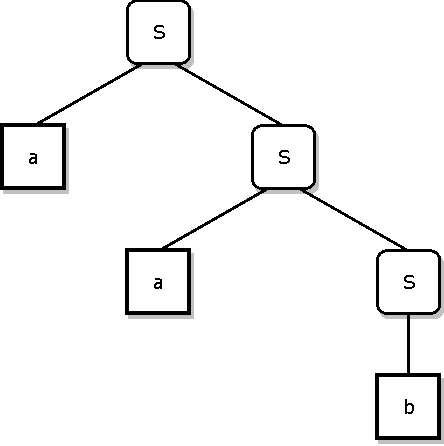
\includegraphics[width=5cm]{img/DerivacniStromDemo}
				\caption{Ukázka derivačního stromu}
			\end{figure}
		
			\paragraph{Nejednoznačné slovo}
			je takové slovo, pro které existuje v gramatice několik různých derivačních stromů. Pro příklad uveďme gramatiku obsahující sčítání a odčítání
			\Grammar{a,+,-}{S}{S}{S\rightarrow S+S,\allowbreak S\rightarrow S-S,\allowbreak S\rightarrow a} kde díky nejednoznačnosti není pevně dána přednost operací u slova $w=a+a-a$ (viz obrázek \ref{pic:ambiguousTree}).
			\begin{figure}[h!]
				\centering
				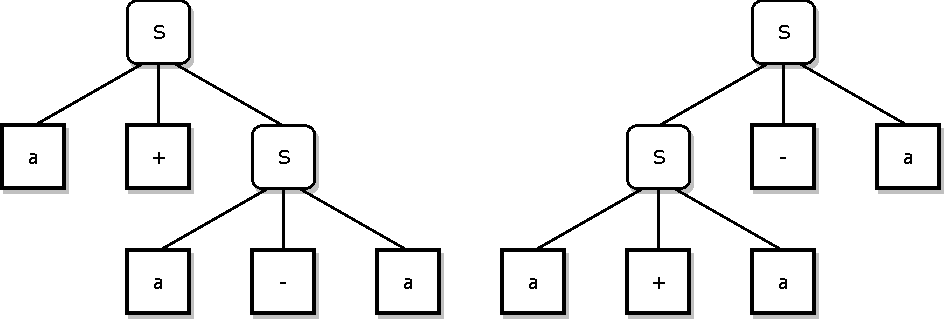
\includegraphics[width=10cm]{img/NejednoznacnyDerivacniStrom}
				\caption{Derivační stromy pro nejednoznačné slovo}
				\label{pic:ambiguousTree}
			\end{figure}
			\paragraph{Jednoznačná gramatika}
			je taková gramatika, která nemá v~generujícím jazyce ani jedno nejednoznačné slovo.
			
		
		\subsection{Deterministické bezkontextové gramatiky}
			Deterministické gramatiky, nebo také \LRk gramatiky, jsou gramatiky ekvivalentní s~modelem deterministického zásobníkového automatu. Jedná se o~podmnožinu jednoznačných gramatik \cite{Meduna:2014:FLC:2636678}. Jak již bylo řečeno, zásobníkový automat je model, který byl přiřazen právě k~bezkontextovým gramatikám jako jejich ekvivalent -- dokážou popsat stejnou množinu jazyků. Následující popis vychází z~materiálu \cite{Meduna:2014:FLC:2636678}.
			
			\paragraph{Deterministický stavový automat}
			je pětice $M=\left(Q, T, \delta, q_0, F\right)$. $Q$ je množina vnitřních stavů, $T$ je vstupní abeceda (ekvivalent terminálů), $\delta$ je zobrazení $Q\times X\rightarrow Q$, $q_0$ je počáteční stav automatu ($q_0\in Q$) a $F$ je množina koncových stavů. Automat na základě aktuálního stavu a dalšího znaku na vstupu přechází do stavu jiného, a to podle zobrazení $\delta$. Tento proces končí až ve chvíli, kdy je přečteno celé slovo. Pokud není pro vstupní symbol definována přechodová funkce, proces končí a říkáme, že automat slovo nepřijal. Pokud je po přečtení celého slova automat v~jednom z~koncových stavů (množina $F$), potom tvrdíme, že automat slovo přijal.
			\paragraph{Nedeterministický stavový automat}
			je deterministický stavový automat, pouze s~rozdílnou definicí zobrazení $\delta$. Pro jeho nedeterministickou verzi je zobrazení $\delta$ definováno jako $Q\times T\rightarrow {2}^{Q}$, kde ${2}^{Q}$ je potenční množina. To znamená, že na základě stavu a následujícího znaku vstupního slova může automat přejít do více stavů současně. Pro další znak slova se provádí stejný postup pro každý jednotlivý stav, a to nezávisle na ostatních stavech. Netederministický stavový automat slovo přijímá, jestliže alespoň jedna z~větví skončila v~koncovém stavu.
			\paragraph{Nedeterministický zásobníkový automat}
			je automat definovaný sedmicí $K=\left(Q, T, Z, \delta, q_0, Z_0, F\right)$. Od stavového automatu se liší abecedou zásobníku $Z$, počátečním symbolem zásobníku $Z_0 \in Z$ a pravidly $\delta$ tvaru $Q \times (T \cup \left\{\varepsilon\right\}) \times \theta_S \rightarrow Q \times \theta_E$ kde $\theta_S, \theta_E \in  {Z}^{\ast}$. Přechod probíhá na základě aktuálního stavu, dalšího znaku vstupního slova ~ na základě libovolného explicitního počtu znaků na zásobníku $\theta_S$. Tyto znaky jsou ze zásobníku odebrány, automat se přesune do nového stavu a vloží na zásobník libovolný (i~nulový) počet znaků $\theta_E$.\par
			Stejně jako u nedeterministického stavového automatu, paralelní přechody jsou na sebe navzájem nezávislé, tj. operace se zásobníkem u jednoho přechodu neovlivní stav zásobníku u zbylých přechodů. Automat končí ve chvíli, kdy není definována přechodová funkce, nebo kdy je přečteno celé vstupní slovo. Automat má dvě možnosti, jak může slovo přijmout. Stejně jako u~nedeterministického stavového automatu, nedeterministický zásobníkový automat slovo příjímá, jestliže jedna z~větví skončí v~koncovém stavu. Automat taktéž slovo přijímá, pokud alespoň jedna větev odebrala ze zásobníku všechny symboly a~přečetla celé vstupní slovo. O~tom, kterým způsobem nedeterministický zásobníkový automat slovo přijímá, se musíme rozhodnout při definici automatu.
			\paragraph{Deterministický zásobníkový automat}
			je zásobníkový automat, pro kte\-rý existuje v~každém stavu maximálně jeden přechod, a to pro libovolný vstupní symbol i pro libovolné slovo na zásobníku.
			Nedeterminismus u zásobníkového automatu je způsoben situací, při níž existují přechody vycházející ze stejného stavu na stejný vstupní symbol (resp. symbol \Eps), a sekvence symbolů $\theta_{S1}$ jednoho přechodu je předponou sekvence $\theta_{S2}$ přechodu druhého. Pro příklad uveďme přechody $(Q_1 , a , Z_1) = (Q_2 , \varepsilon)$ a $(Q_1 , a , Z_1 Z_2 ) = (Q_2 , \varepsilon)$. Je-li automat ve stavu $Q_1$, na vstupu je symbol $a$ a na zásobníku jsou symboly $Z_1 Z_2$, potom vyhovují oba přechody a zásobník se stává nedeterministickým.
			Stejně jako u~jeho nedeterministické verze, deterministický zásobníkový automat slovo přijímá, jestliže přečte celé slovo a~skončí v~koncovém stavu, nebo přečte-li celé slovo a~ze zásobníku odebere všechny symboly. Způsob přijetí je nutný definovat předem.
			\paragraph{Deterministické bezkontextové gramatiky}
			jsou gramatiky, pro které lze sestrojit deterministický zásobníkový automat.
			
			\vspace{1em}
			
			Determinismus u zásobníkového automatu je pro \LRk gramatiky (resp. \LRk parsery) klíčový. Dovoluje totiž parsování v~lineárním čase v~závislosti na délce slova. \LRk parsery byly prvně popsány Donald Knuthem,
			ale bylo od nich opuštěno z~důvodu velkých paměťových nároků na parsovací algoritmus. S~ohledem na zvyšující se výkon počítačů se k~tomuto algoritmu opět vracíme \cite{Chapman:1987:LPT:40693}.
			
			Pro libovolnou deterministickou bezkontextovou gramatiku lze sestrojit \LRk parser, jedná se tedy o nejuniverzálnější parser s~lineární časovou složitostí. Pro parsování je použita tzv. bottom-up metoda založená právě na fungování deterministického zásobníkového automatu \cite{Chapman:1987:LPT:40693}. 
			
			Zjednodušeně se na zásobník postupně vkládají znaky vstupního slova. Ve chvíli, kdy existuje pravidlo, které se derivuje na symboly v~zásobníku, je pravidlo použito a~symboly v~zásobníku jsou nahrazeny levou stranou pravidla. Tento postup nutně nemusí vést na deterministický zásobníkový automat. Aby kompiler věděl, které pravidlo použít, používá tzv. \MathSymb{LR parsing table}. Ta je předpočítaná a obsahuje vyhovující pravidla v závislosti na dalších znacích vstupního slova. Parser na základě \MathSymb{k} nepřečtených znaků vstupního slova a~aktuálního stavu zásobníku vyhledá v tabulce příslušné pravidlo, které použije (odtud \LRk parsery). Tím je zajištěn determinismus a lineární časová složitost \cite{Meduna:2014:FLC:2636678}. 
		
		\subsection{LL gramatiky}
			\label{sec:LLgrammars}
			\LLk gramatiky \cite{Blythe:1994:LLV:191033.191121} jsou podobně jako \LRk gramatiky založeny na fungování deterministického zásobníkového automatu, ale tentokrát tzv. top-down metodou. Ta nejprve vloží na zásobník startovací symbol. Existuje-li pravidlo, které přepisuje symbol na vrcholu zásobníku, je použito a symbol na zásobníku je nahrazen pravou stranou pravidla. Ve chvíli, kdy je symbol na vstupu stejný jako symbol na vrcholu zásobníku, je symbol ze zásobníku odebrán a~symbol ze vstupu přečten.
			
			Tento postup téměř jistě nevede na deterministický zásobníkový automat, protože je symbol expandován bez znalosti vstupu (tedy nedeterministicky). Proto \LLk parsery (podobně jako \LRk parsery) tvoří tzv. \MathSymb{LL parsing table}, která plní stejnou funkci (odtud \LLk parsery).
			
			\LLk gramatiky nejsou tak univerzální jako \LRk gramatiky (jsou jejich podmnožinou), protože se při parsování musí rozhodnout o~použití pravidla ještě před tím, než je jakýkoliv vstup přečten (na rozdíl od \LRk parserů, které se rozhodují až po přečtení). Na druhou stranu se díky tomu v \MathSymb{LL parsing table} zajímáme pouze o levou stranu pravidel, zatímco v \MathSymb{LR parsing table} je to strana pravá. To vede k menšímu počtu záznamů a~tím k~menší zátěži na paměť \cite{Blythe:1994:LLV:191033.191121}.
		
		\subsection{LR(0), \gls{gloss:SLR} a \gls{gloss:LALR} gramatiky}
			\MathSymb{LR(0)}, \MathSymb{SLR} a \MathSymb{LALR} gramatiky jsou zjednodušení \LRk gramatik \cite{Chapman:1987:LPT:40693}. Ačkoliv dokáže \LRk gramatika zpracovat libovolnou deterministickou gramatiku, paměťová složitost \LRk parserů byla v~minulosti příliš velká. \MathSymb{LR(0)} parsery fungují bez paměťové režie (parsery mají nulový náhled, tedy \MathSymb{LR parse table} není použita), ale mají malou vyjadřovací schopnost.
			
			Z~toho důvodu popsal Frank DeRemer dvě zjednodušené verze \LRk parserů, konkrétně Simple LR Parser (\MathSymb{SLR}) a~Look-Ahead LR Parser (\MathSymb{LALR}) \cite{Deremer:1969:PTL:888578}.
			Tyto parsery si ponechaly lineární časovou složitost, ale na rozdíl od \LRk parserů jsou méně náročné na paměť.
			
		\vfill
			
		Vzhledem k počtu skupin, které byly výše zmíněny, je přiložen graf (obrázek \ref{pic:contextfreeLanguages}) ukazující bezkontextové gramatiky, jejich rozdělení a vzájemnou inkluzi a~exkluzi jednotlivých podmnožin.
		
		\begin{figure}[h]
			\centering
			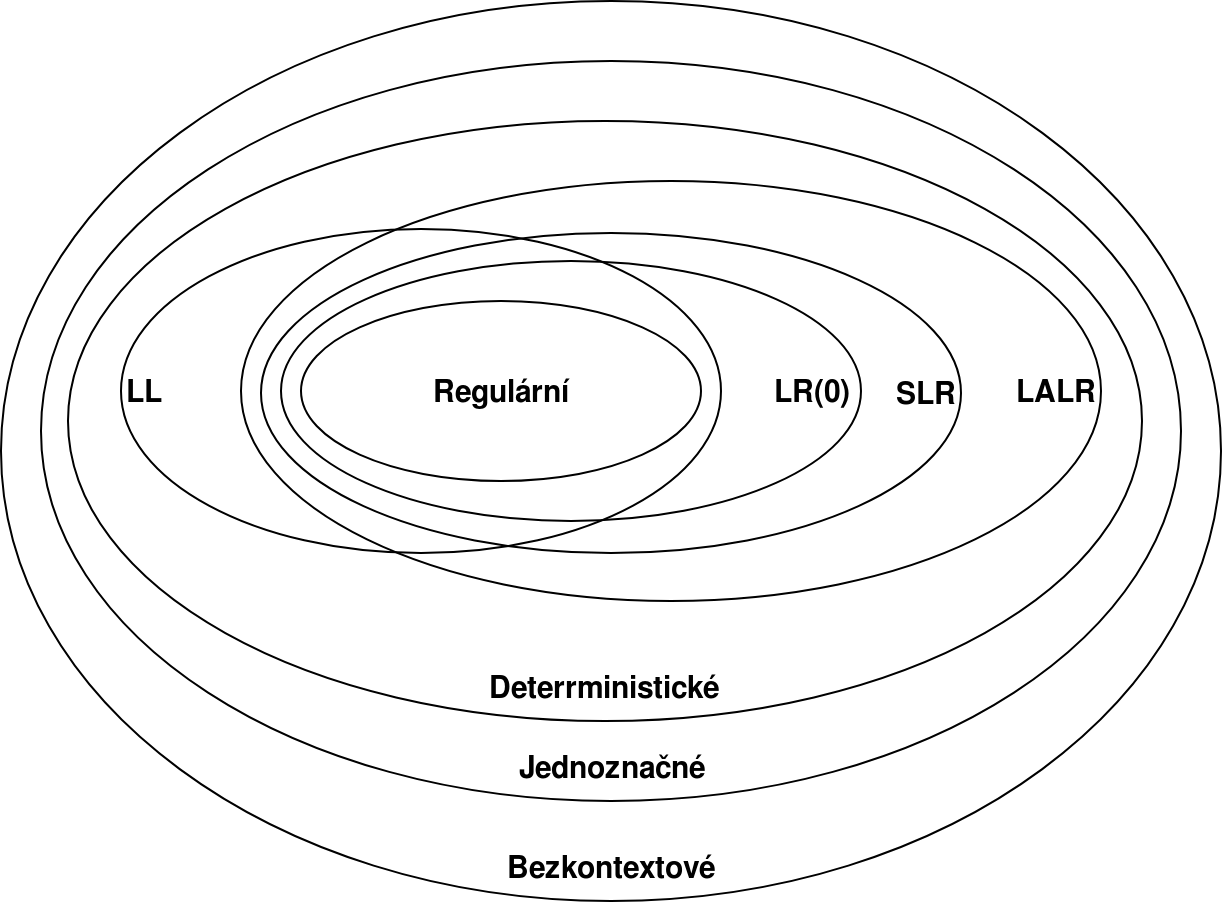
\includegraphics[width=8cm]{img/ContextFreeLanguageGroups}
			\caption{Rozdělení bezkontextových jazyků}
			\label{pic:contextfreeLanguages}
		\end{figure}
		
		S~již zmíněnými parsovacími metody se nebudeme dále zabývat, protože nejsou předmětem této práce. Byly vyjmenovány z důvodu, že na ně knihovna musí pamatovat pro budoucí rozšíření. Práce se dále zabývá \gls{gloss:CYK} algoritmem, který je detailněji popsán v~daůší části. Pro použití \gls{gloss:CYK} algoritmu je nutné mít gramatiku v~\gls{gloss:CNF} a~tomu se věnuje sekce \ref{sec:ChomskyNormalForm}.
		
	\section{Formální překlady}
		Překlad \cite{Aho:1969:TCF:800169.805425} je operace, která každému vstupu přiřazuje nějaký výstup. Překlady mezi různými světovými jazyky pravděpodobně není nutné zmiňovat, ale může se jednat i~o~převod matematických zápisů mezi prefixovou, postfixovou a~infixovou notací. Dalším příkladem je převod mezi číselnými soustavami nebo kódování (například binární data na Base64).
		
		\paragraph{Fomální překlad}
		je relace $Z\subseteq L\times V$, kde $L$ je libovolný jazyk a $V$ jazyk překladů. Relace přiřazuje každému slovu jazyka \MathSymb{L} jeho překlad patřící do \MathSymb{V}.
		\paragraph{Překladová gramatika}
		je \TranslateGrammarDef, \MathSymb{T} je množina terminálů (resp. vstupních symbolů), \MathSymb{N} je množina neterminálů, \MathSymb{D} je výstupní abeceda (disjunktní s~abecedou terminálů a~neterminálů), \MathSymb{S} je počáteční symbol a \MathSymb{R} je množina pravidel $R\subseteq{\left(T \cup N \cup D\right)}^{\ast}$.
		
		\vspace{1em}
		
		Do definice gramatik přibyla v~překladové gramatice výstupní abeceda (či množina výstupních symbolů). Výstupní symboly budeme dále v~textu označovat malými písmeny v~kruhu -- \circled{a}, \circled{x}.
		
		\paragraph{Homomorfismus}
		je zobrazení $h\subseteq X \times Y^\ast$, kde \MathSymb{X} a \MathSymb{Y} jsou abecedy.
		\paragraph{Rozšířený homomorfismus}
		je homomorfismus $h:X^*\times Y^*$ definovaný indukcí.
		$$h(\varepsilon)=\varepsilon$$
		$$h(xa)=h(x)h(a), x\in X^*, a\in X$$		
		\paragraph{Vstupní homomorfismus}
		je rozšířený homomorfismus, který nahrazuje všechny symboly $x\in D$ symbolem \Eps.
		\paragraph{Výstupní homomorfismus}
		je rozšířený homomorfismus, který nahrazuje všechny symboly $x\in T \cup N$ symbolem \Eps.
		
		\vspace{1em}
		
		Překlad zpravidla probíhá tak, že je naparsováno vstupní slovo (odtud vstupní homomorfismus) a podle použitých pravidel je výsledkem výstupní slovo (odtud výstupní homomorfismus). Samotný derivační strom (resp. větná forma) obsahuje jak vstupní, tak výstupní symboly.
		
		Předpokládejme \TranslateGrammarNoRuleSet{a,+,*}{S,A,P,K}{\circled{a},\circled{+},\circled{-}}{S}{R}, kde R:
		\begin{center}
			\begin{minipage}{.45\textwidth}
				\begin{lstlisting}[escapeinside={(*}{*)}]  
S (*$\rightarrow$*) a(*\circled{a}*)A
S (*$\rightarrow$*) a(*\circled{a}*)
K (*$\rightarrow$*) a(*\circled{a}*)(*\circled{$\ast$}*)A
K (*$\rightarrow$*) a(*\circled{a}*)(*\circled{$\ast$}*)
				\end{lstlisting}
			\end{minipage}
			\hfill
			\begin{minipage}{.45\textwidth}
				\begin{lstlisting}[escapeinside={(*}{*)}]  
A (*$\rightarrow$*) (*$\ast$*)Kz
A (*$\rightarrow$*) +P
P (*$\rightarrow$*) a(*\circled{a}*)(*\circled{+}*)A
P (*$\rightarrow$*) a(*\circled{a}*)(*\circled{+}*)
				\end{lstlisting}
			\end{minipage}
		\end{center}
	
		Pro vstupní slovo $w_i=a + a \ast a$ bude překlad $w_o=\circled{a}\circled{a}\circled{+}\circled{a}\circled{$\ast$}$. Derivační strom je v~příloze na obrázku \ref{fig:translateGrammar}.
		
		Ačkoliv by se to z~názvu \enquote{Překladové gramatiky} dalo usuzovat, tyto gramatiky ve skutečnosti nepřekládají programy do spustitelné podoby. Překladové gramatiky nejsou schopny dodat sémantickou stránku překladu, tedy to, jak se bude program chovat. K tomu slouží gramatiky atributované.
		
	\section{Atributované gramatiky}
		Již zmiňované parsovací metody řeší pouze skladbu vstupního slova -- jeho syntax. Jeho skladba má ovšem i~specifický význam -- hovoříme o~sémantickém významu. Následující kapitola vychází primárně z~materiálu \cite{4308414}.
		
		\paragraph{Syntax}
		je množina pravidel a principů, které řídí strukturu věty daného jazyka, zpravidla definicí povolených kombinací symbolů. Syntax zajišťuje ověření, zda je vstupní věta správně strukturována.
		
		\vspace{1em}
		
		Správnou syntaxi vstupní věty vynutíme právě použitím gramatik. Ve většině případů nechceme pouze ověřit, zda je vstupní věta syntakticky správně, ale požadujeme její další zpracování. Pokud již máme vytvořenou syntaxi, nezpracováváme samotný text, ale jeho význam. Z~tohoto důvodu se snažíme text během procesu parsování převést do jiných struktur, vhodnějších pro další zpracování. Jednou z~takových struktur je abstraktní syntaktický strom.
		
		\paragraph{Abstraktní syntaktický strom}
		je stromovou reprezentací abstraktní syntaktické struktury zdrojového kódu. Uzly abstraktního derivačního stromu reprezentují konstrukce ve zdrojovém kódu. Abstraktní syntaktický strom dodržuje pravidla syntaxe, uzly a hrany derivačního stromu jsou převedeny do struktur vhodných k~dalšímu zpracování. Samotná podoba těchto struktur se může v~závislosti na dalším zpracování lišit. Svým způsobem se jedná o~reprezentaci derivačního stromu datovými strukturami. Abstraktní syntaktický strom budeme dále v textu označovat jako \gls{gloss:AST} (z~anglického Abstract Syntax Tree).
		
		\vspace{1em}
			
		Abstraktní syntaktický strom reprezentuje syntaktickou stránku programovacích jazyků. Respektuje správnou syntax, ale nedefinuje význam, tedy sémantiku. Sémantika musí být přidána dodatečně.
		
		\paragraph{Sémantika}
		přidává význam syntakticky korektním větám. V kontextu programovacích jazyků sémantika popisuje postup, který zařízení provádí během spuštění daného programu.
		
		\vspace{1em}
		
		Pro definici atributované gramatiky, která dodává sémantický význam, potřebujeme nadefinovat další pojmy.
		
		\paragraph{Atribut}
		je veličina, která může nabývat hodnot z~definované množiny. Atribut můžeme přirovnat k~proměnné v~programovacích jazycích.
		\paragraph{Atributovaný symbol}
		je symbol abecedy, ke kterému je přiřazena konečná množina atributů. Tato množina může být i prázdná. Přístup k~atributu $a$ přiřazeného symbolu $x$ budeme značit jako $x.a$. Atribut $a$ s hodnotou \MathSymb{1} pro symbol $x$ budeme značit jako $x.a[1]$. Jestliže bude atributů více, budeme je oddělovat tečkou, tedy symbol $x$ s jeho atributy $a=1$ a $b=2$ budeme značit jako $x.a[1].b[2]$.
		\paragraph{Atributovaný řetězec}
		nad abecedou $A$ je řetězec atributovaných symbolů z~$A$.
		\paragraph{Atributovaný překlad}
		je relace ${T}^{\ast} \times {D}^{\ast}$, kde ${T}^{\ast}$ je množina vstupních atributovaných řetězců a ${D}^{\ast}$ množina výstupních atributovaných řetězců.
		
		\vspace{1em}
		
		Vztáhneme-li kontext zpět na gramatiky a~\gls{gloss:AST}, můžeme každému terminálu a~neterminálu přiřadit množinu atributů. Dále budeme uvažovat pouze o jednom atributu \MathSymb{v}. Pomocí atributů můžeme mít několik způsobů, jak reprezentovat číslo 253.
		\begin{itemize}
			\item Neterminál $x$ reprezentující celé číslo jako $x.v[253]$.
			\item Neterminál $x$ reprezentující cifru a pravidla $c \rightarrow x c, c\rightarrow\varepsilon$, kde $c$ reprezentuje celé číslo. Pro číslo 253 by 
			$c\Rightarrow x_1c \Rightarrow x_1x_2c\Rightarrow x_1x_2x_3c\Rightarrow x_1x_2x_3$, kde $x_1.v[2], x_2.v[5], x_3.v[3]$.
			\item Neterminály $x_0,x_1,\cdots,x_9$ s pevně danými atributy $x_k.v[k]$.
		\end{itemize}
	
		Konkrétní výběr se může lišit podle způsobu dalšího zpracování a kontextu gramatiky. Z~pohledu sémantiky bychom ovšem potřebovali, abychom ke všem třem variantám přistupovali stejně, tedy očekáváme, že kořen \gls{gloss:AST} reprezentující číslo bude mít atribut obsahující hodnotu čísla. Přitom chceme zůstat nezávislí na způsobu reprezentace.
		
		Jak je z~popisu patrné, hodnoty neterminálních atributů nemůžeme volit pevně, ale musí se měnit v závislosti na pozici v~\gls{gloss:AST} -- nejčastěji na základě atributů potomků nebo rodiče. Toho dosáhneme sémantickými pravidly.
		
		\paragraph{Sémantická funkce}
		je funkce, která přiřadí atributu hodnotu na základě jiných atributů. Jedná se o funkci $f=(a_1,a_2,\cdots,c_n)$, kde $a_1,a_2,\cdots,c_n$ jsou atributy, na kterých je funkce závislá. Funkce je zapsána libovolným, pro danou situaci vhodným způsobem (například programovacím jazykem uvnitř překladače).
		\paragraph{Sémantické pravidlo}
		je pravidlo, které má navíc sémantickou funkci.
		\paragraph{Atributovaná překladová gramatika}
		je \AttributTranslateGrammarDef, kde \MathSymb{N} je abeceda neterminálů, \MathSymb{T} je abeceda terminálů, \MathSymb{D} je abeceda výstupních symbolů, \MathSymb{SR} jsou sémantické pravidla, \MathSymb{S} je počáteční symbol $S\in N$, \MathSymb{A} je množina atributů a \MathSymb{V} je zobrazení $V\subseteq\left(T\cup N\right)\times{A}^\ast$, tedy množina přiřazující každému terminálu či neterminálu množinu atributů.
		\paragraph{Dědičný atribut}
		je atribut \MathSymb{v} symbolu \MathSymb{x}, jehož sémantická funkce \MathSymb{f} závisí pouze na dědičných atributech symbolu \MathSymb{x} nebo na dědičných atributech jeho rodiče.
		\paragraph{Syntetizovaný atribut}
		je atribut \MathSymb{v} symbolu \MathSymb{x}, jehož sémantická funkce závisí pouze na syntetizovaných či dědičných atributech symbolu \MathSymb{x}, nebo na syntetizovaných či dědičných atributech jeho potomků.
		\paragraph{Vyhodnocení atributů}
		je proces, během kterého jsou vyhodnoceny sémantické funkce a nastaveny hodnoty atributů. Pro správné vyhodnocení musí být splněno:
		\begin{itemize}
			\item hodnoty dědičných atributů počátečního symbolu musí být známy,
			\item hodnoty syntetizovaných atributů vstupních symbolů musí být známy,
			\item hodnota atributu musí záviset pouze na již známých hodnotách atributů.
		\end{itemize}
		
		\vspace{1em}
		
		Poslední bod vylučuje situace, které by mohly vést k~zacyklení výpočtu. Nejjednodušším příkladem je atribut \MathSymb{a} závisející na atributu \MathSymb{b}, přitom atribut \MathSymb{b} zpětně závisí na atributu \MathSymb{a}. Pokud budou atributy záviset pouze na již známých hodnotách atributů, k~zacyklení dojít nemůže.
		
		Jako příklad atributované gramatiky uvedeme gramatiku vyhodnocující aritmetické operace \MathSymb{+} a \MathSymb{$\ast$}. Pro všechny symboly předpokládáme syntetizovaný atribut \MathSymb{v}. Pravidla lze nalézt v~tabulce \ref{tab:attributed_arithmetic}. Symboly, které se v~pravidlu vykytují opakovaně je nutné v~sémantických funkcích rozlišit, proto jsou symboly indexovány. V~obrazové příloze je na obrázku \ref{fig:attributedGrammar} zobrazeno vyhodnocení vstupního slova $a.v[3]+a.v[2]*a.v[4]$.
		
		\begin{table}[h!]
			\centering
			\caption{Atributovaná gramatika vyhodnocující aritmetické operace}	
			\label{tab:attributed_arithmetic}
			\begin{tabular}{| l | l |}
				\hline
				\textbf{Pravidlo} & \textbf{Sémantika} \\
				\hline
				\MRule{S}{E} & $S.v = E.v$ \\
				\hline
				\MRule{E_1}{E_2 + T} & $E_1.v = E_2.v + T.v$ \\
				\hline
				\MRule{E}{T} & $E.v = T.v$ \\
				\hline
				\MRule{T_1}{T_2 * F} & $T_1.v = T_2.v * F.v$ \\
				\hline
				\MRule{T}{F} & $T.v = F.v$ \\
				\hline
				\MRule{F}{a} & $F.v = a.v$ \\
				\hline
				\MRule{F}{\left(E\right)} & $F.v = E.v$ \\
				\hline
			\end{tabular}		
		\end{table}
		
	\section{Chomského normální forma}
		\label{sec:ChomskyNormalForm}
		Chomského normální forma (\gls{gloss:CNF}) je speciální formát gramatiky vyžadována \gls{gloss:CYK} algoritmem. Libovolnou bezkontextovou gramatiku lze převést do \gls{gloss:CNF} \cite{Meduna:2014:FLC:2636678}.
		Pro tuto transformaci jsou známy a popsány algoritmy, které jsou blíže rozebrány v~další kapitole.
		
		Chomského normální forma povoluje pouze pravidla následujících typů:
		\begin{itemize}
			\item $A \rightarrow B C$,
			\item $A \rightarrow a$,
			\item $S \rightarrow \varepsilon$, kde \Nonterm{S} se nesmí vyskytovat na pravé straně žádného pravidla.
		\end{itemize}
	
		Před tím, než blíže popíšeme algoritmy pro transformaci gramatik, sloužící k~převodu do \gls{gloss:CNF}, potřebujeme dodefinovat další pojmy, které se v~kontextu těchto transformací vyskytují. Pojmy vycházejí z~materiálu \cite{Meduna:2014:FLC:2636678}.
		
		\paragraph{Negenerující symbol}
		je symbol, který negeneruje žádnou větu. Pokud je počáteční symbol \MathSymb{S} negenerující, gramatika negeneruje žádné slovo, a~tedy generuje prázdný jazyk.
		\paragraph{Dostupný symbol}
		je symbol, který se vyskytuje v~nějaké větné formě. Formálně se jedná o symbol $X: S \Rightarrow\alpha X \beta; \alpha,\beta\in\TermNontermIter$.
		\paragraph{Nedostupný symbol}
		je symbol, který není dostupný.
		\paragraph{\EpsS pravidlo}
		je pravidlo ve tvaru $X\rightarrow\varepsilon$.
		\paragraph{Zkracující pravidlo}
		je pravidlo, jehož počet symbolů na levé straně je větší než počet symbolů na straně pravé. Délka \EpsS symbolu je považována za nulovou.
		\paragraph{Zkracující gramatika}
		je gramatika, která má alespoň jedno pravidlo zkracující.
		\paragraph{Symbol derivovatelný na \EpsS přímo}
		je takový symbol \MathSymb{X}, pro nějž platí $X{\Rightarrow}^{1}\varepsilon$. V~gramatice musí existovat pravidlo $X\rightarrow\varepsilon$.
		\paragraph{Symbol derivovatelný na \EpsS nepřímo}
		je takový symbol \MathSymb{X}, pro nějž platí $X{\Rightarrow}^{i}\varepsilon;i>1$.
		\paragraph{Jednoduché pravidlo}
		je pravidlo tvaru $A \rightarrow B$, tedy pravidlo přepisující neterminál na neterminál.
		
		
		
	